\documentclass{article}
	\usepackage{ctex}
    \usepackage{geometry}
        \geometry{left=2.54cm,right=2.54cm,top=2.54cm,bottom=2.54cm}
    \usepackage{graphicx}
    \usepackage{subfig}
    \usepackage{float}
    \begin{document}
	\title{\textbf{信号与系统大作业} \\ [2ex] \begin{large} \emph{小白鲸找妈妈} \end{large} }
	\author{王晗\\(2013011076)}
	\date{\today}
	\maketitle
	\section{单频信号模拟}
		\subsection{读入whalesong.wav文件,听一听声音;绘制波形,解释波形和声音的关系}
            whalesong.wav波形如下图所示:
            \begin{figure}[htb]
                \centering
                \subfloat[完整波形]
                {
                    \label{fig:origin-1}
                    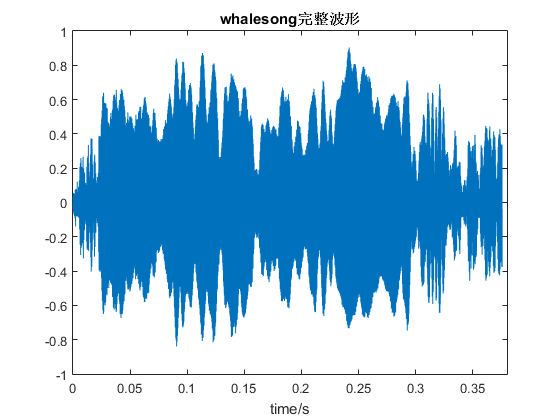
\includegraphics[width=7cm]{figure1.png}
                }
                \hspace{10pt}
                \subfloat[局部波形]
                {
                    \label{fig:origin-2}
                    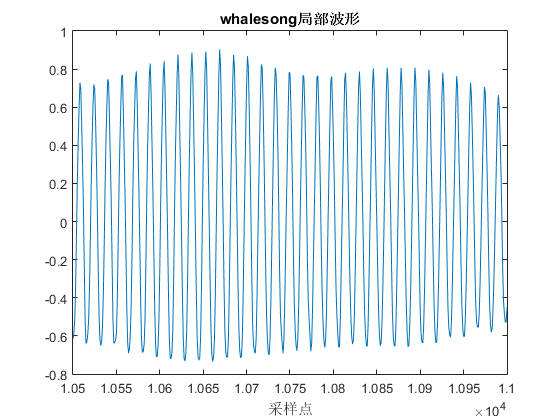
\includegraphics[width=7cm]{figure2.png}
                }
                \caption{whalesong波形}
                \label{fig:origin}
            \end{figure}
            
            将波形和实际的音频进行比较,可以发现波形振幅的表示声音的响度,波形的振动频率表示声音的频率。

        \subsection{如果要用一个单频信号模拟上述声音,请计算该信号的频率}
            由局部波形图计算,采样点$1.05\times10^4$ $\sim$ $1.095\times10^4$之间共有28个周期,采样频率44.1kHz,故单频信号频率:
            $$f=\frac{1}{\frac{(1.095-1.05)\times10^4}{44.1\times10^4\times28}}Hz=2744Hz$$
            
        \subsection{由计算得到的频率合成一个单频信号,绘制波形,听听声音,解释和白鲸的歌声有何异同}
            合成音频波形如下图所示:
            \begin{figure}[htb]
                \centering
                \subfloat[完整波形]
                {
                    \label{fig:output1-1}
                    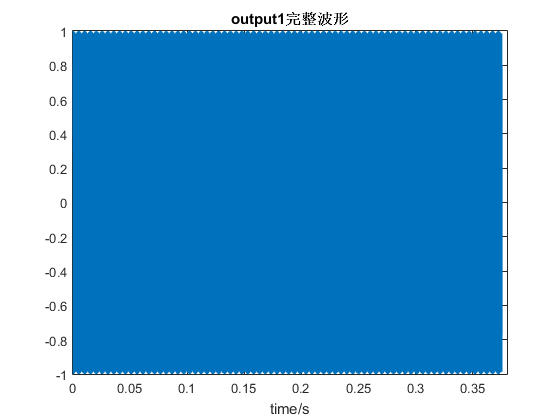
\includegraphics[width=7cm]{figure3.png}
                }
                \hspace{10pt}
                \subfloat[局部波形]
                {
                    \label{fig:synfixed-2}
                    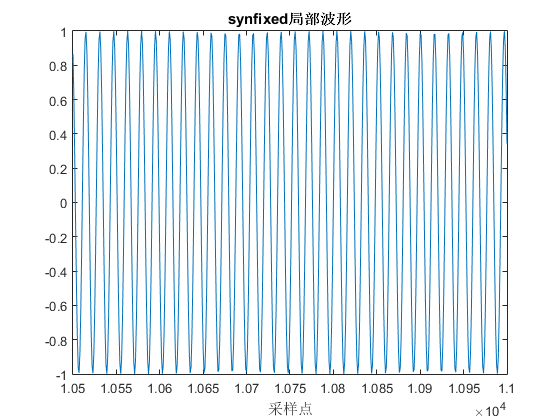
\includegraphics[width=7cm]{figure4.png}
                }
                \caption{synfixed波形}
                \label{fig:synfixed}
            \end{figure}
            
            单频模拟出的声音和白鲸的叫声差别较大,单频信号听起来干涩、单薄、缺乏变化,而白鲸的歌声较为饱满、通透。
            
        \subsection{将上述单频信号保存为synfixed.wav文件}
    
    \section{变频信号模拟}
        \subsection{读入whalesong.wav文件,绘制时频图,解释其含义}
            \begin{figure}[htb]
                \centering
                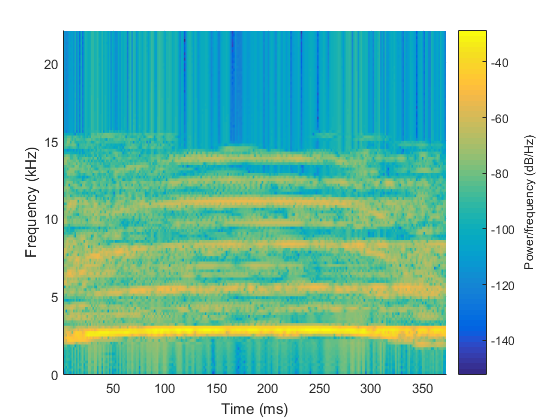
\includegraphics[width=9cm]{figure5.png}
                \label{fig:originft-1}\caption{Matlab绘制的whalesong时频图}
            \end{figure}
            
            \begin{figure}[!htb]
                \centering
                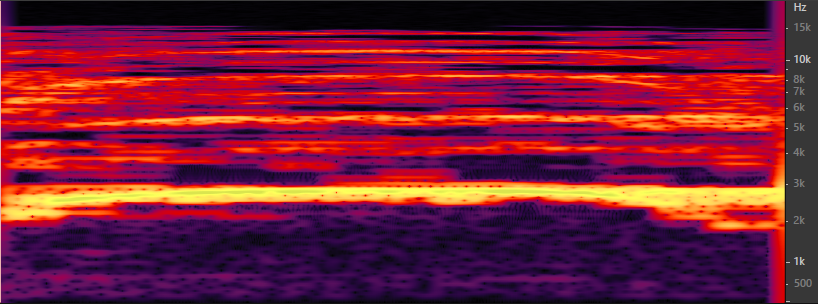
\includegraphics[width=10cm]{figure6.png}
                \label{fig:originft-2}\caption{Audition绘制的whalesong时频图}
            \end{figure}
            
            时频图中的颜色分布表示不同时间点上能量在频域的分布,颜色越量的区域能量越高。上图表明白鲸叫声的能量在频域主要分布在若干个频率附近。
            
        \subsection{如果要用一个包络和频率都随时间变化的单频信号模拟上述声音,请描述该频率变化的特征}
            1$\sim$4000采样点频率由2.25kHz线性增加至2.8kHz,幅度由0.2线性增加至1;12000$\sim$16572采样点频率由2.8kHz线性降低至1.94kHz,幅度由1线性降低至0。
            
        \subsection{用上题结果合成一个变频信号,绘制波形和时频图,听听声音,解释和白鲸的歌声有何异同}
            合成音频波形如下图所示:
            \begin{figure}[htb]
                \centering
                \subfloat[完整波形]
                {
                    \label{fig:synsingle-1}
                    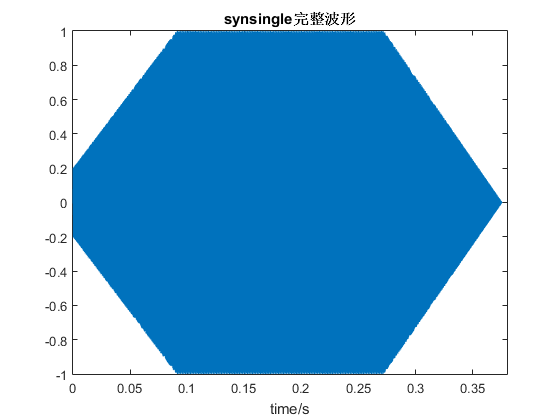
\includegraphics[width=7cm]{figure7.png}
                }
                \hspace{10pt}
                \subfloat[局部波形]
                {
                    \label{fig:synsingle-2}
                    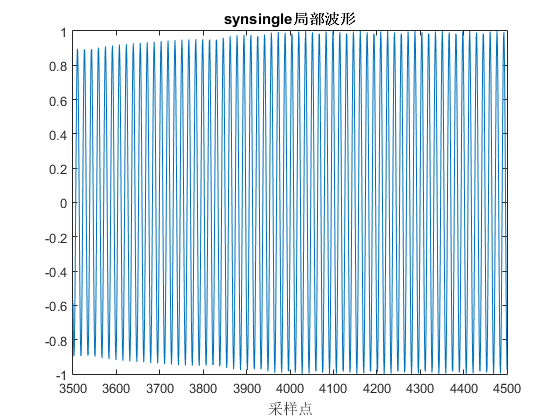
\includegraphics[width=7cm]{figure8.png}
                }
                \caption{synsingle波形}
                \label{fig:synsingle}
            \end{figure}
            
            时频图:
            \begin{figure}[H]
                \centering
                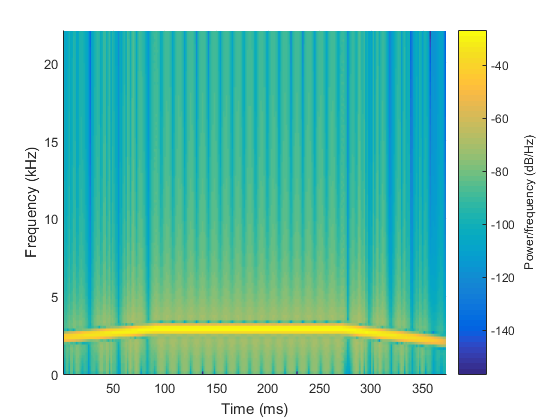
\includegraphics[width=9cm]{figure9.png}
                \label{fig:synsingle-ft}\caption{synsingle时频图}
            \end{figure}
            
            现在合成的音频在响度、基频变化等方面已经比较接近白鲸的叫声了,但是由于缺少高频分量,声音显得单薄、苍白。
            
        \subsection{将上述变频信号保存为synsingle.wav文件}
        
    \section{多变频信号模拟}
        \subsection{认真观察whalesong的时频图,思考什么结构的合成信号能更好的模拟它}
        
\end{document} 